\documentclass[a4paper]{article}

\usepackage{fullpage} % Package to use full page
\usepackage{parskip} % Package to tweak paragraph skipping
\usepackage{tikz} % Package for drawing
\usepackage{amsmath}
\usepackage{amsfonts}
\usepackage{amssymb}
\usepackage{hyperref}
\usepackage[utf8]{inputenc}
\usepackage[english]{babel}
\usepackage{multicol}

\newcommand\tab[1][0.5cm]{\hspace*{#1}}

\def\firstcircle{(0:1cm) circle (1cm)}
\def\secondcircle{(180:2.5cm) circle (2.5cm)}
\def\thirdcircle{(0:2.5cm) circle (2.5cm)}
\def\fourthcircle{(135:2.5cm) circle (2.5cm)}
\def\fifthcircle{(45:2.5cm) circle (2.5cm)}
\def\sixthcircle{(270:1.3cm) circle (2.5cm)}
\usetikzlibrary{matrix,shapes.geometric}
\setlength{\columnsep}{-4cm}

\title{Discrete Mathematics: HW4}
\author{Adrian Darian}
\date{2018/10/03}

\begin{document}

\maketitle

\section*{1.8 Proof Method and Strategy}
\begin{itemize}
  \item[16] Show that if $a, b,$ and $c$ are all real numbers and $a \neq 0$, then there is a unique solution of the equation $ax + b = c$. \\
  $ax = c - b$ \\
  $x = (c - b) / a$ \\
  As long as $a \neq 0$ there always exists a unique solution
  \item[44] Prove or disprove that you can use dominoes to tile a $5 x 5$ checkerboard with three corners removed. \\
  \begin{multicols}{2}
    \tikzstyle{checker} = [cylinder, minimum width=.8cm, 
    shape border rotate=90,cylinder end fill=gray!50!white,
    cylinder body fill=gray, cylinder uses custom fill]
    \begin{tikzpicture}
      \draw[ultra thick] (0,0) rectangle (5,-5);
          \foreach \row in {0,1, ..., 4} {
              \foreach \column in {0, 1.5} {
          \fill ({2*\column + mod(\row,2)}, -\row) rectangle +(1,-1);
              }
          }
      \matrix (m) at (0,0) [matrix of nodes,nodes=checker,
        anchor=north west,column sep={1cm,between origins},
        row sep={1cm,between origins}] {
        {1} & {2} & {3} & {4} & {5}  \\
        {6} & {7} & {8} & {9} & {10} \\
        {11} & {12} & {13} & {14} & {15} \\
        {16} & {17} & {18} & {19} & {20} \\
        {21} & {22} & {23} & {24} & {25} \\
        };
    \end{tikzpicture} \\
    There are 13 black squares and 12 white squares, assuming we remove 3 of the corners from the grid we now have 10 black squares and 12 white squares. Since we cannot cover the whole board with checkers due to the number of black and white squares not equaling out. Our required result is found.
  \end{multicols}
\end{itemize}

\section{2.1 Sets}
\begin{itemize}
  \item[16] Use a Venn diagram to illustrate the relationships $A \subset B$ and $A \subset C$. \\ \\
  \begin{tikzpicture}
    \draw \firstcircle node [text=black,above left] {$A$};
    \draw \secondcircle node [text=black,above right] {$B$};
    \draw \thirdcircle node [text=black,below] {$C$};
  \end{tikzpicture} \\ \\
  \item[20] What is the cardinality of each of these sets? \\
    a. $\emptyset$ \\
    \tab $|\emptyset| = 0$ \\
    c. $\{ \emptyset, \{\emptyset\}\}$ \\
    \tab $|\{\emptyset, \{\emptyset\}\}| = 2$
  \item[24] Determine whether each of these sets is the power set of a set, where $a$ and $b$ are distinct elements. \\
    b. $\{\emptyset, \{a\}\}$ \\
    \tab For a set $A$ if $|A| = k$ $\therefore$ the cardinality of $P(A) = 2^k$ \\
    \tab There is only $1$ element in $A = \{a\}$, so the cardinality of $P(A) = 2^1 = 2$ \\
    \tab $\{a\}$ is a power set of $\{\emptyset, \{a\}\}$ \\
    \tab Thus $A = \{a\}$ is a power set \\
    c. $\{\emptyset, \{a\}, \{\emptyset, a\}\}$ \\
    \tab There is only $1$ element in $A = \{a\}$, so the cardinality of $P(A) = 2^1 = 2$ \\
    \tab However this cannot be a power set, $\therefore$ the given set is not a power set.
  \item[26] Show that if $A \subseteq C$ and $B \subseteq D$, then $A x B \subseteq C x D$ \\
  \tab $A x B = \{(a, b)|a \in A, b \in B\}$ \\
  \tab $C x D = \{(c, d)|c \in C, d \in D\}$ \\
  \tab If $a \in A \rightarrow a \in C$ as $A \subseteq C$ and $b \in B \rightarrow b \in D$ as $B \subseteq D$ \\
  \tab Let $(a, b) \in A x B \rightarrow (a, b) \in C x D$ for all $a \in A$ and all $b \in B$ \\
  \tab $\therefore A x B \subseteq C x D$
  \item[32] Let $A = \{a, b, c\}$, $B = \{x, y\}$, and $C = \{0, 1\}$. Find \\
    a. $A x B x C$ \\
    \tab $A x B x C = \{(a, x, 0), (a, x, 1), (a, y, 0), (a, y, 1), (b, x, 0), (b, x, 1), (b, y, 0), (b, y, 1), (c, x, 0), (c, x, 1), (c, y, 0), (c, y, 1)\}$ \\
    b. $C x B x A$ \\
    \tab $C x B x A = \{(0, x, a), (0, x, b), (0, x, c), (0, y, a), (0, y, b), (0, y, c), (1, x, a), (1, x, b), (1, x, c), (1, y, a), (1, y, b), (1, y, c)\}$
  \item[38] Show that $A x B \neq B x A$, when $A$ and $B$ are nonempty, unless $A = B$. \\
  \tab $A x B = \{(x, y)|x \in A \land y \in B\}$ \\
  \tab $A \neq B$ \\
  \tab $a \in A \land a \notin B$ or $b \in B \land b \notin A$ \\
  \tab $(a, b) \in A x B$, but $(b, a) \notin A x B$ while $a \notin B$ \\
  \tab $b \in B \land a \in A$ gives you $(b, a) \in B x A$ \\
  \tab $(b, a) \notin A x B$ and $(b, a) \in B x A$ \\
  \tab $A x B \neq B x A$
  \item[44] Find the truth set of each of these predicates where the domain is the set of integers. \\
    b. $Q(x): x^2 = 2$ \\
    \tab Truth set is $\emptyset$ \\
    c. $R(x): x < x^2$ \\
    \tab Truth set is $-\{0, 1\}$
\end{itemize}

\section*{2.2 Set Operations}
\begin{itemize}
  \item[4] Let $A = \{a, b, c, d, e\}$ and $B = \{a, b, c, d, e, f, g, h\}$. Find \\
    c. $A - B$ \\
    \tab $A - B = \emptyset$ \\
    d. $B - A$ \\
    \tab $B - A = \{f, g, h\}$
  \item[18] Let $A, B$, and $C$ be sets. Show that \\
    c. $(A - B) - C \subseteq A - C$ \\
    \tab $(A - B) - C = \{x|x \in (A - B) \land x \notin C\}$ by definition of intersection and difference \\
    \tab\tab\tab\tab\tab $= \{x|(x \in A \land x \notin B) \land x \notin C\}$ by definition of difference\\
    \tab\tab\tab\tab\tab $= \{x|(x \in A \land (\neg x \in B)) \land (\neg x \in C)\}$ by definition of does not belong symbol \\
    \tab\tab\tab\tab\tab $= \{x|x \in A \land (\neg x \in B) \land (\neg x \in C)\}$ \\
    \tab If $x \in A \land (\neg x \in B) \land (\neg x \in C)$ then $x \in A \land (\neg x \in C)$ \\
    \tab Thus, $\{x|x \in A \land (\neg x \in B) \land (\neg x \in C)\} \subseteq \{x|x \in A \land (\neg x \in C)\}$ \\
    \tab $(A - B) - C = \{x|x \in A \land (\neg x \in B) \land (\neg x \in C)\}$ \\
    \tab\tab\tab\tab\tab $\subseteq \{x|x \in A \land (\neg x \in C)\}$ \\
    \tab\tab\tab\tab\tab $\subseteq \{x|x \in A \land (x \notin C)\}$ by definition of does not belong symbol \\
    \tab\tab\tab\tab\tab $\subseteq \{x|x \in A - C\}$ by definition of difference \\
    \tab\tab\tab\tab\tab $= A - C$ by meaning of set builder notation \\
    \tab $\therefore (A - B) - C \subseteq A - C$ \\
    d. $(A - C) \cap (C - B) = \emptyset$ \\
    \tab $(A - C) \cap (C - B) = \{x|x \in (A - C) \land x \in (C - B)\}$ by definition of intersection \\
    \tab\tab\tab\tab\tab $= \{x|(x \in A) \land (x \notin C) \land (x \in C) \land (x \notin B)\}$ by definition of difference \\
    \tab\tab\tab\tab\tab $= \{x|(x \in A) \land (\neg x \in B) \land (x \in C) \land (\neg x \in C)\}$ by definition of not belong symbol \\
    \tab\tab\tab\tab\tab $= \{x|((x \in A) \land (\neg x \in B)) \land ((x \in C) \land (\neg x \in C))\}$ by definition of associative \\
    \tab\tab\tab\tab\tab $= \{x|((x \in A) \land (\neg x \in B)) \land ((x \in C -C))\}$ by definition of difference \\
    \tab\tab\tab\tab\tab $= \{x|((x \in A) \land (x \notin B)) \land x \in \emptyset\}$ by definition of not belong symbol \\
    \tab\tab\tab\tab\tab $= \{x|(x \in A - B) \land x \in \emptyset\}$ by definition of intersection \\
    \tab\tab\tab\tab\tab $= \{x \in (A - B) \cap \emptyset\}$ by definition of set builder notation \\
    \tab\tab\tab\tab\tab $= (A - B) \cap \emptyset$ by defintion of domination law \\
    \tab\tab\tab\tab\tab $= \emptyset \therefore (A - C) \cap (C - B) = \emptyset$
  \item[24] Let $A, B$, and $C$ be sets. Show that $(A - B) - C = (A - C) - (B - C)$. \\
  \tab $(A - C) - (B - C) = \{x|x \in (A - C) \land x \notin (B - C)\}$ by the definition of difference of two sets \\
  \tab $(A - C) - (B - C) = \{x|x \in (A - C) \land x \in \overline{(B - C)}\}$ by definition of complement of sets \\
  \tab $(A - C) - (B - C) = \{x|x \in (A \cap \overline{C}) \land x \in \overline{(B \cap \overline{C})}\}$ since $A - C = A \cap \overline{C}$ and $B - C = B \cap \overline{C}$ \\
  \tab $(A - C) - (B - C) = \{x|x \in (A \cap \overline{C}) \land x \in (\overline{B} \cup C)\}$ by DeMorgan's law and complementation law \\
  \tab $(A - C) - (B - C) = \{x|x \in (A \cap \overline{C}) \cap (\overline{B} \cup C)\}$ by definition of intersection of two sets \\
  \tab $(A \cap \overline{C}) \cap (\overline{B} \cup C) = D \cap (\overline{B} \cup C)$ by taking $A \cap \overline{C} = D$ \\
  \tab $(A \cap \overline{C}) \cap (\overline{B} \cup C) = (D \cap \overline{B}) \cup (D \cap C)$ by distributive laws \\
  \tab $(A \cap \overline{C}) \cap (\overline{B} \cup C) = ((A \cap \overline{C}) \cap \overline{B}) \cup ((A \cap \overline{C}) \cap C)$ since $A \cap \overline{C} = D$ \\
  \tab $(A - C) - (B - C) = \{x|x \in (A \cap \overline{C}) \cap (\overline{B} \cup C)\}$ \\
  \tab $(A - C) - (B - C) = \{x|x \in ((A \cap \overline{C}) \cap \overline{B}) \lor x \in ((A \cap \overline{C}) \cap C)\}$ by defintion of union of two sets \\
  \tab $(A - C) - (B - C) = \{x|x \in ((A \cap (\overline{C} \cap \overline{B})) \lor x \in (A \cap (\overline{C} \cap C))\}$ by associative law \\
  \tab $(A - C) - (B - C) = \{x|x \in (A \cap (\overline{B} \cap \overline{C})) \lor x \in (A \cap \phi)\}$ by commutative law and complement law \\
  \tab $(A - C) - (B - C) = \{x|x \in (A \cap \overline{B}) \cap \overline{C} \lor x \in \phi\}$ by associative law \\
  \tab $= \{x|x \in (A - B) \cap \overline{C}\}$ since $A - B = A \cap \overline{B}$ \\
  \tab $= \{x|x \in (A - B) - C\}$ since $(A - B) - C = (A - B) \cap \overline{C}$ \\
  \tab $= (A - B) - C$ by the meaning of set builder notation \\
  \tab $\therefore (A - C) - (B - C) = (A - B) - C$
  \item[26] Draw the Venn diagrams for each of these combinations of the sets $A, B$, and $C$. \\
    b. $\overline{A} \cap \overline{B} \cap \overline{C}$ \\
    \tab by DeMorgan's Law $\overline{A} \cap \overline{B} = \overline{A \cup B}$\\
    \tab $\overline{A \cup B \cup C}$ \\ \\
    \begin{tikzpicture}
      \draw \fourthcircle node [text=black,above left] {$A$};
      \draw \fifthcircle node [text=black,above right] {$B$};
      \draw \sixthcircle node [text=black,below] {$C$};
    \end{tikzpicture} \\ \\
    c. $(A - B) \cup (A - C) \cup (B - C)$ \\
    \tab $(A \cap \overline{B}) \cup (A \cap \overline{C}) \cup (B \cap \overline{C})$ \\
    \tab $\{(A \cap \overline{B}) \cup (A \cap \overline{C})\} \cup \{(A \cap \overline{C}) \cup (B \cap \overline{C})\} (\because X \cup X = X)$ \\
    \tab by Distributive property $\{A \cap (\overline{B} \cup \overline{C})\} \cup \{\{A \cup B\} \cap \overline{C}\}$ \\ \\
    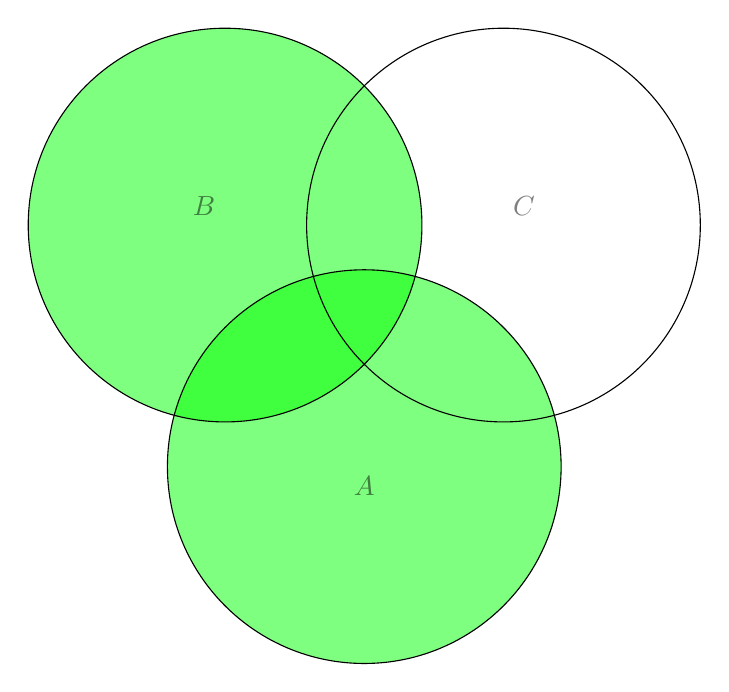
\begin{tikzpicture}
      \begin{scope}[fill opacity=0.5]
        \fill[green] \fourthcircle;
        \fill[green] \sixthcircle;
        \draw \fourthcircle node [text=black, above left] {$B$};
        \draw \fifthcircle node [text=black, above right] {$C$};
        \draw \sixthcircle node [text=black, below] {$A$};
      \end{scope}
    \end{tikzpicture}
\end{itemize}

\end{document}